\item Let $\vec{A}$ be a $3 \times 3$ real matrix having eigenvalues 1, 2, and 3. If $\vec{B}= \vec{A}^2 + 2\vec{A} + \vec{I}$,
where $\vec{I}$ is the $3 \times 3$ identity matrix, then the eigenvalues of $\vec{B}$ are

\hfill(2023 XE)

\begin{multicols}{4}

\begin{enumerate}

\item 4, 9, 16

\item 1, 2, 3

\item 1, 4, 9

\item 4, 16, 25

\end{enumerate}

\end{multicols}
\item If the polynomial
$$P\brak{x} = a_0 + a_1 x + a_2 x\brak{x-1} + a_3 x\brak{x-1}\brak{x-2}$$
interpolates the points $\brak{0,2}, \brak{1,3}, \brak{2,2}$ and $\brak{3,5}$, then the value of $P\brak{\frac{5}{2}}$ is \underline{\hspace{1cm}}.

\hfill(2023 XE)
\item Let  $\vec{P} = \myvec{4 & -2 & 2\\ 6 & -3 & 4\\ 3 & -2 & 3}$ and $\vec{Q} = \myvec{3 & -2 & 2\\ 4 & -4 & 6\\ 2 & -3 & 5}$.
The eigenvalues of both $\vec{P}$ and $\vec{Q}$ are $1, 1, 2$. Which one of the following
statements is TRUE?
\hfill(2023 XE)
\begin{multicols}{2}
\begin{enumerate}
\item Both $\vec{P}$ and $\vec{Q}$ are diagonalizable
\item $\vec{P}$ is diagonalizable but $\vec{Q}$ is NOT diagonalizable
\item $\vec{P}$ is NOT diagonalizable but $\vec{Q}$ is diagonalizable
\item Both $\vec{P}$ and $\vec{Q}$ are NOT diagonalizable
\end{enumerate}
\end{multicols}
\item A block of mass $m=10$ kg is lying on an inclined plane $PQ$. The mass is
restrained from sliding down the inclined plane by a force $\vec{F}$. The coefficient of
friction between the block and the inclined plane is 0.3. Take the acceleration due
to gravity as 10 m/s$^2$. The smallest force $\vec{F}$ \brak{in N} required to prevent the block
from sliding down is \rule{1cm}{0.01pt}.
\hfill(2023 XE)
\begin{figure}[H]
\centering
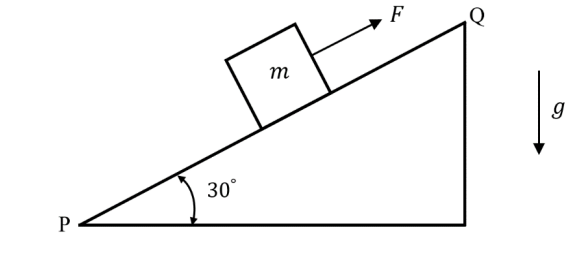
\includegraphics[width=0.5\columnwidth]{GATE/2023/XE/figs/fig14.png}
\caption{}
\label{fig:figs/C/fig14.png/2023}
\end{figure}

